\chapter{Radiation in Bending Magnets}\label{bendrad}
Considering radiation effects is crucial during the design stage of an accelerator, where effects can be evaluated by tracking particles through the lattice or by analytical approximations. However, during the design process this effect is measured iteratively after lattice optic parameters are set. In order to include both, radiation and optic parameters, during the design optimization process, radiation in bending magnets is reviewed in this chapter.\par
The theory developed by Sands in \cite{Sands} is first presented in order to clarify all terms used in the beam size contribution from the radiation model. The analytical result is generalized to the case with non-zero phase advance at the IP and non-zero dispersion, required during the optimization process. The closed solution for one dipole and one dipole with a drift is compared with the tracking code PLACET \cite{Placet} and finally the model validity for the FFS design is analyzed.
\section{Theoretical approximation}\label{radtheo}
Assuming a lattice that can be described by transport matrices in the form written in the Eq. (\ref{eq-matrix}), radiation effects can be calculated by the model in  \cite{Sands}.
\begin{equation}
\begin{pmatrix}
x_2\\
x'_2\\
\delta
\end{pmatrix}
=
\begin{pmatrix}
 C(s_1,s_2) & S(s_1,s_2)& R_{16}(s_1,s_2)\\
 C'(s_1,s_2) & S'(s_1,s_2) & R_{26}(s_1,s_2)\\
 0 & 0 &1
\end{pmatrix}
\begin{pmatrix}
x_1\\
x'_1\\
\delta
\end{pmatrix}
\label{eq-matrix}
\end{equation}
Being $\Delta x_i = R_{16}(s_i,s_p) (-u)/E$, the deviation at the observation point $s_p$ due to the $i^{\text{th}}$ photon of energy $u$ radiated at some point $s_i$, and $E$ the beam energy.\par The first rhs term in Eq. (\ref{eq-sumphot}) is the sum over the $N$ photons radiated during the time $T$ for the particle to cross the magnet. $N(T)$ describes the probability distribution of photon emission. As we are interested only in the second order moment, the mean  $x_0=\langle\sum_{i=1}^{N(T)}\Delta x_i\rangle$ is subtracted from the sum, obtaining $\langle x\rangle=0$, $ \sigma_{bend}^2=\langle x^2\rangle$, being $x$ the horizontal transverse displacement from the reference orbit of a particle at the observation point.
\begin{equation}
\sum_{i=1}^{N(T)}\Delta x_i - x_0 = x\label{eq-sumphot}
\end{equation}
The photon emission follows a Poisson distribution as a consequence of the normalized radiation spectrum and photon number spectrum of synchrotron radiation used in \cite{Sands2} Section 5. For any Poisson-like distribution $\sigma_N^2 = \langle N\rangle$. The beam size contribution due to radiation has two components of variability: the spread of $\Delta x_i$ due to the energy emission $u$ and the number of times the emission process occurs $N$\footnote{Using statistics notation, $\sigma_x=V(x)$ and $\langle x\rangle=E(x)$, then, a process with two components of variability has a variance expressed as $V(x)=E(V(x|N))+V(E(x|N))$. The term $(x|N)$ denotes the evaluation of the $x$ variable for a given $N$}. Therefore, it is calculated as in Eq. (\ref{eq-bsize})
\begin{align}
\sigma^2_{bend} &= \langle x^2\rangle - \cancelto{0}{\langle x\rangle^2} = \langle x^2 \rangle\label{eq-bsize}\\
 &= \langle N\rangle \sigma^2_{\Delta x} + \langle \Delta x \rangle ^2 \sigma_N^2\\
 &= \langle N\rangle \langle (\Delta x)^2\rangle -\cancel{\langle N\rangle\langle\Delta x\rangle^2} + \cancel{\langle \Delta x \rangle^2\langle N \rangle}\\
 &=\langle N\rangle \langle (\Delta x)^2\rangle
\end{align}
Where the $i$ sub-index has been removed intentionally because the photon number emission is extracted from a continuous function of $u$ the photon energy and either $T$ or $s/c$, where $c$ is the speed of light.\par 
The rate of emission of photons is calculated as in Eq. (\ref{eq-nu}) where $K_{5/3}$ is the modified Bessel function, $u_c=\frac{3}{2}\frac{\hbar c \gamma^3}{\rho}$ called the critical energy which depends on the relativistic factor $\gamma$, the reduced Planck constant $\hbar$ and the particle trajectory curvature $\rho$, and $P_\gamma=\frac{2cr_emc^2}{3\rho^2}\gamma^4$ is the instantaneous radiated power where $r_e$ is the classical electron radius and $m$ is the electron mass.
\begin{equation}
n(u,s)=\frac{P_\gamma}{u_c^2}\left[\frac{9\sqrt{3}}{8\pi}\int_{u/u_c}^\infty K_{5/3}(\xi) d\xi\right]\label{eq-nu}
\end{equation}
Using $\Delta x(s) = (-u/E) R_{16}(s,s_p)$ the second moment is calculated by integration over the entire space and energies.
\begin{align}
 \sigma_{bend}^2&=\int_0^{T} \int_0^\infty [\Delta x(u,s)]^2 n(u,s)dudT\label{eqDeltaX}\\
 &=\frac{1}{c}\int_0^{s_p} \int_0^\infty \left[\frac{-u}{E}R_{16}(s,s_p)\right]^2 n(u,s)duds\\
\end{align}
Finally, 
\begin{equation}
\sigma^2_{bend}=C_2\int_0^{s_p} \frac{E^5}{\rho^3}R_{16}(s,s_p)^2 ds\label{eq-R16}
\end{equation}
where $C_2=\frac{55}{24\sqrt{3}}\frac{r_e\hbar c}{(mc^2)^6}=4.13\times10^{-11} \text{ m}^2\text{GeV}^{-5}$ is a constant coming from the emission rate integration already derived by Sands.\par
\subsection{Generalization for the optimization process}\label{s:thebeamrad}
During the optimization process it is convenient to rewrite $R_{16}$ using the off-momentum function $\eta$, lattice parameters and Eq. (\ref{eq-matrix}). Measuring from the reference orbit, the kick propagation from $s$ to $s_p$ can be written in terms of the general transport matrix, giving
\begin{align}
\Delta x(s)_{total}=\frac{-u}{E}\eta(s_p) &= \frac{-u}{E} \left[C(s,s_p)\eta(s) + S(s,s_p)\eta'(s) + R_{16}(s,s_p)\right]\\
\eta(s_p) &= \sqrt{\frac{\beta_{s_p}}{\beta_s}}\left[\eta_s\cos\Delta\phi_{s,s_p}+(\alpha_s\eta_s+\beta_s\eta'_s)\sin\Delta\phi_{s,s_p}\right] + R_{16}(s,s_p)\label{eq-disp}
\end{align}
where $\alpha, \beta$ and $\phi$ are the optics parameters and the subscripts indicate the evaluation point. The equations derived by Sands in \cite{Sands} assume $\alpha_{s_p}=0, \eta_{s_p}=0$ and $\eta'_{s_p}=0$, which are not valid during the lattice optimization process nor in the case of waist shift to get more luminosity in ILC and CLIC \cite{PhysRevSTAB.16.041001}.\par
From Eq. (\ref{eq-R16}) and (\ref{eq-disp}) is clear that the contribution to beam size due to radiation now can be calculated as:
\begin{equation}
 \sigma_{bend}^2=C_2 \int_0^{s_p} \frac{E^5_s}{\rho^3_s}\left\{\sqrt{\frac{\beta_{s_p}}{\beta_s}}\left[\eta_s\cos\Delta\phi_{s,s_p}+(\alpha_s\eta_s+\beta_s\eta'_s)\sin\Delta\phi_{s,s_p}\right]-\eta_{s_p}\right\}^2ds\label{eq-radbends}
\end{equation}
Eq. (\ref{eq-radbends}) was included in MapClass2 in order to be used during lattice design and optimization. It is also worth noting that $\eta_{s_p}=0$ agrees with the result obtained by Sands in the ideal case with zero dispersion at the IP. This generalized expression I obtained is solved for the simple case of one bending magnet and compared with tracking results.

\subsection{One dipole and one dipole with a drift}
An analytical closed expression has been derived for the case of one sector magnet ($\rho,L,\theta$) and a sector magnet plus a drift ($L_{drift}$). Beam energy loss is negligible compared with beam energy $E$.\par
For a sector magnet, $R_{16}= \rho(1-\cos\theta)$, the radiation effect is calculated as follows
\begin{align}
\sigma_{bend}^2 &= C_2 E^5\int_0^\theta \frac{1}{\rho^3}[\rho(1-\cos(\theta-\chi))]^2\rho d\chi\\
&= C_2E^5\left[\frac{1}{4}(6\theta-8\sin\theta+\sin(2\theta))\right]\label{eqNum}\\
&=C_2E^5\left(\frac{\theta^5}{20}-\frac{\theta^7}{168}+\frac{\theta^9}{2880}-\frac{17\theta^{11}}{1330560}+O(\theta^{13})\right)
\end{align} 
 In the case of a drift after the bending magnet and defining $j=\frac{L_{drift}}{\rho}=\frac{L_{drift}}{L}\theta$
\begin{align}
  \sigma_{bend}^2 =& C_2 \int_0^\theta E^5\left[1-\cos(\theta-\xi)+\frac{L_{drift}}{\rho}\sin(\theta-\xi)\right]^2 d\xi\\
 =& \frac{C_2}{4} E^5 \left[(1-j^2)\sin(2\theta)-8\sin\theta+4j(1-\cos\theta)^2+(6-2j^2)\theta\right]\label{eqNum2}\\
  =& C_2 E^5 \left[\frac{j^2\theta^3}{3}+\frac{j\theta^4}{4}-\frac{(4j^2-3)\theta^5}{60}- \frac{j\theta^6}{24} +\frac{(16j^2-15)\theta^7}{2520}+\frac{j\theta^8}{320}\right.\notag\\
    &-\frac{(64j^2-63)\theta^9}{181440}-\frac{17j\theta^{10}}{120960}+\frac{(256j^2-255)\theta^{11}}{19958400}+\frac{31j\theta^{12}}{7257600}\notag\\
    &\left.-\frac{(1024j^2-1023)\theta^{13}}{3113510400}+O(\theta^{14})\right]
\end{align}
Eqs. (\ref{eqNum}) and (\ref{eqNum2}) will be used to normalize the results from MAPCLASS2 and PLACET \cite{Placet} where some care should be taken due to numerical precision.\par
\section{Comparison of theory and tracking results}\label{s:comparison}
The closed expression is now compared with the general expression included in MAPCLASS2, Eq. (\ref{eq-radbends}), and the tracking code PLACET in the case of one dipole and one dipole and a drift. This can be seen in Fig. (\ref{figSR}), normalized to the close expressions in Eqs. (\ref{eqNum}) and (\ref{eqNum2}), where radiation effect in PLACET was obtained by subtracting the squared beam size from two trackings with same input parameters except for radiation ON/OFF.\par
Figures (\ref{figSR}) (a) and (b) show the effect of systematic change of $\theta$ while keeping $\rho$ and $L$. Figures (\ref{figSR}) (c) and (d) show the effect of changing $L$ while keeping $\rho$ and $\theta$. Figures (\ref{figSR}) (e) and (f) show the effect of changing $L_{drift}$ while keeping the magnet constant. The equivalent magnetic field $B$ is calculated using the magnetic rigidity $B\rho=P/e$ for $E=1.5 $ TeV.\par
When observing the PLACET results, the left side of the plot shows an agreement of (80$\sim$90)\% between the closed expression and the tracking, while the right side shows perfect agreement in almost all cases. The difference is the tracking method used by PLACET.\par
In PLACET 0.99.01 two different implementations of radiation exist: the first is the `default' and the second one will be called  `six\_dim'. `Default' calculates radiation by segmenting the dipole in a \emph{default} number of shorter pieces with Binomial probability of photon emission when the particle traverses each slide. This is called thin dipole approximation and it is also the default tracking method. On the other side, `six\_dim' does not make any sectioning of the dipole, it uses the Poisson probability of photon emission over the entire  dipole, as in the theory.\par
In order to confirm, the authors of PLACET provided several variations of the code where the number of slices was increased, making the Binomial probability to approach the Poisson distribution. Since PLACET 0.99.02 `six\_dim' is the default tracking method.\par
As expected, the MAPCLASS2 and the closed expression are in good agreement, showing the validity of the generalization in Sect. \ref{s:thebeamrad}. %Only Figs. (a) and (b) show abrupt changes at $\theta=7.5\times10^{-7}$ rad due to Twiss result from `ptc\_twiss' 5 dim in MAD-X \cite{MADX}. It is however for very small angles and magnetic fields where a recalculation of the optic parameters using the `twiss' function in MAD-X showed no abrupt changes.\par
There is a point to highlight in Fig. (\ref{figSR}) (b). The tracking, theorical and general calculations are all in good agreement in the range of angles between $10^{-2}$ and $10^{-5}$ rad. Below $10^{-5}$ rad the agreement again decays to (80$\sim$90)\%. This is related to the average number of photons emitted when traversing the dipole and it is explored in Sect \ref{s:modellim}.\par
\begin{figure}[htb]
\centering
  \hspace*{1.2cm}`Default' Synrad\hspace*{5.0cm}Flag `-six\_dim 1'\par
 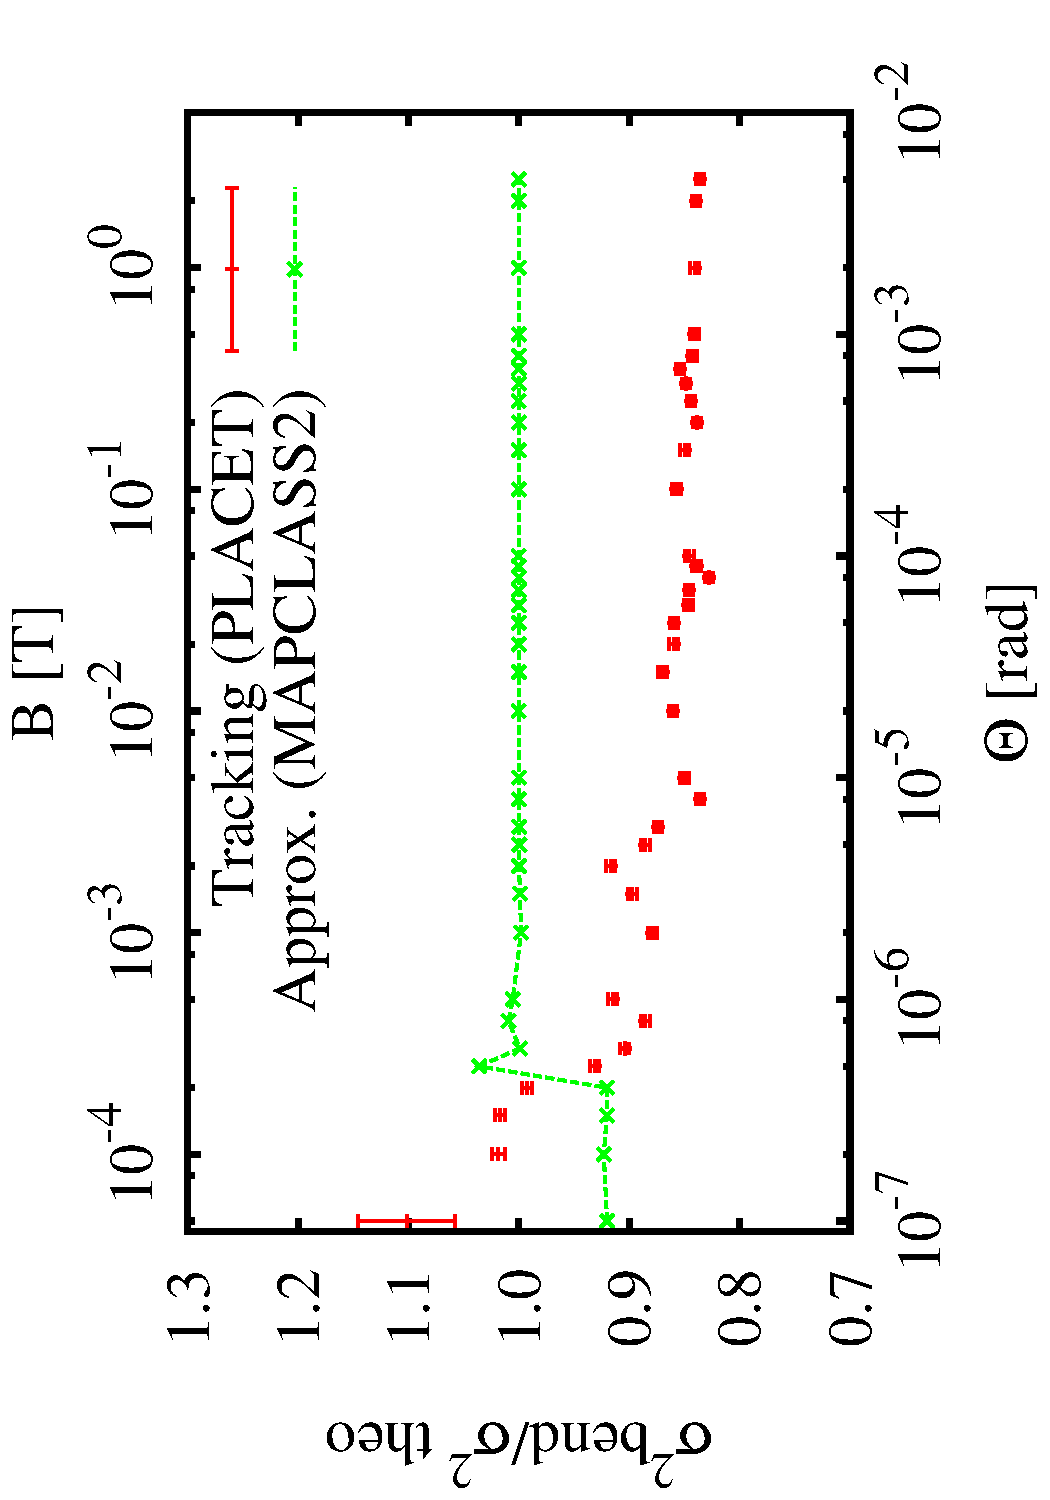
\includegraphics[scale=0.30,angle=-90]{sigma_angle.pdf}
  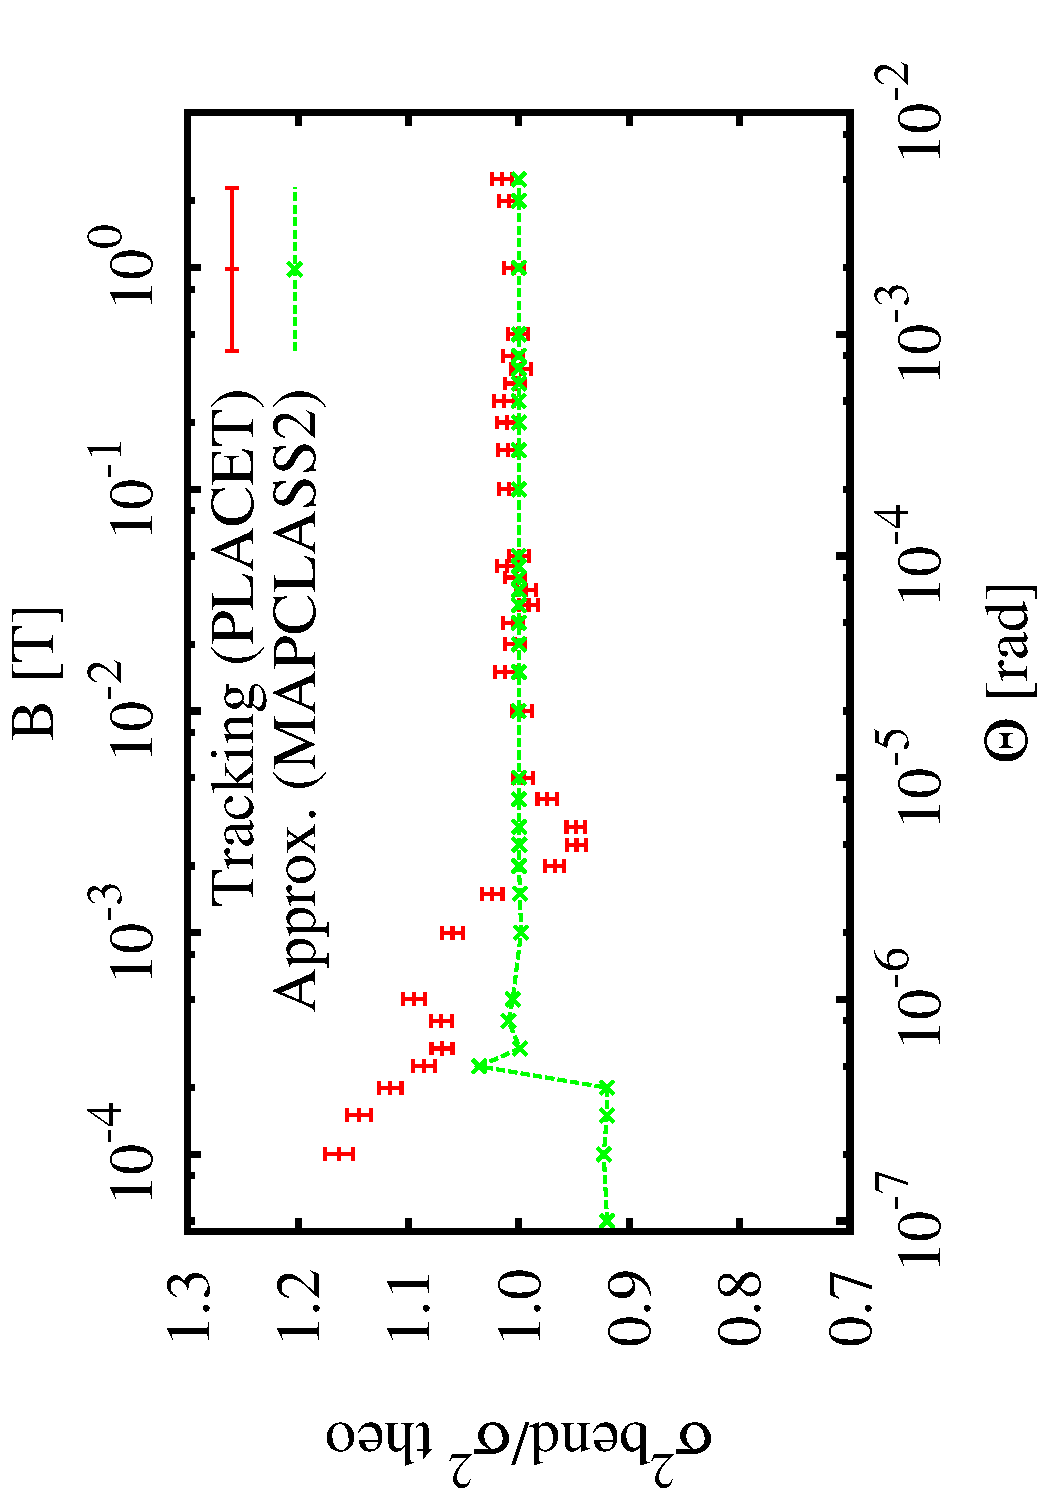
\includegraphics[scale=0.30,angle=-90]{sigma_angle_r06.pdf}\par
%   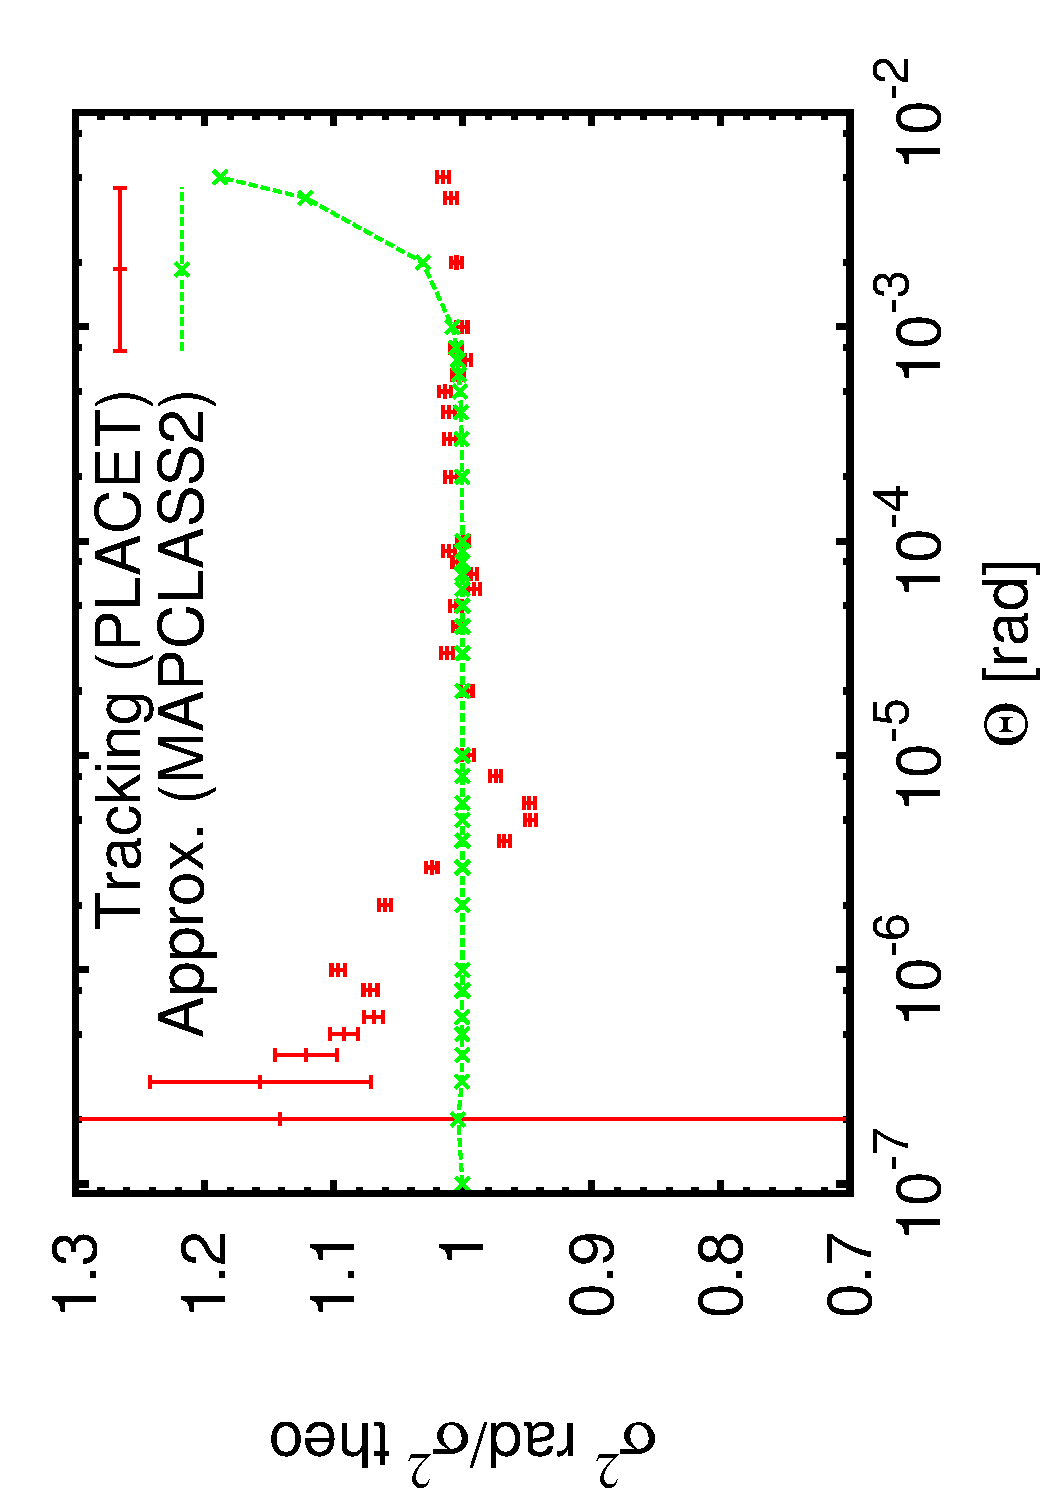
\includegraphics[scale=0.30,angle=-90]{sigma_angle_r6_twiss.pdf}\par
  \hspace*{1.0cm}(a)\hspace*{7.6cm}(b)\par
   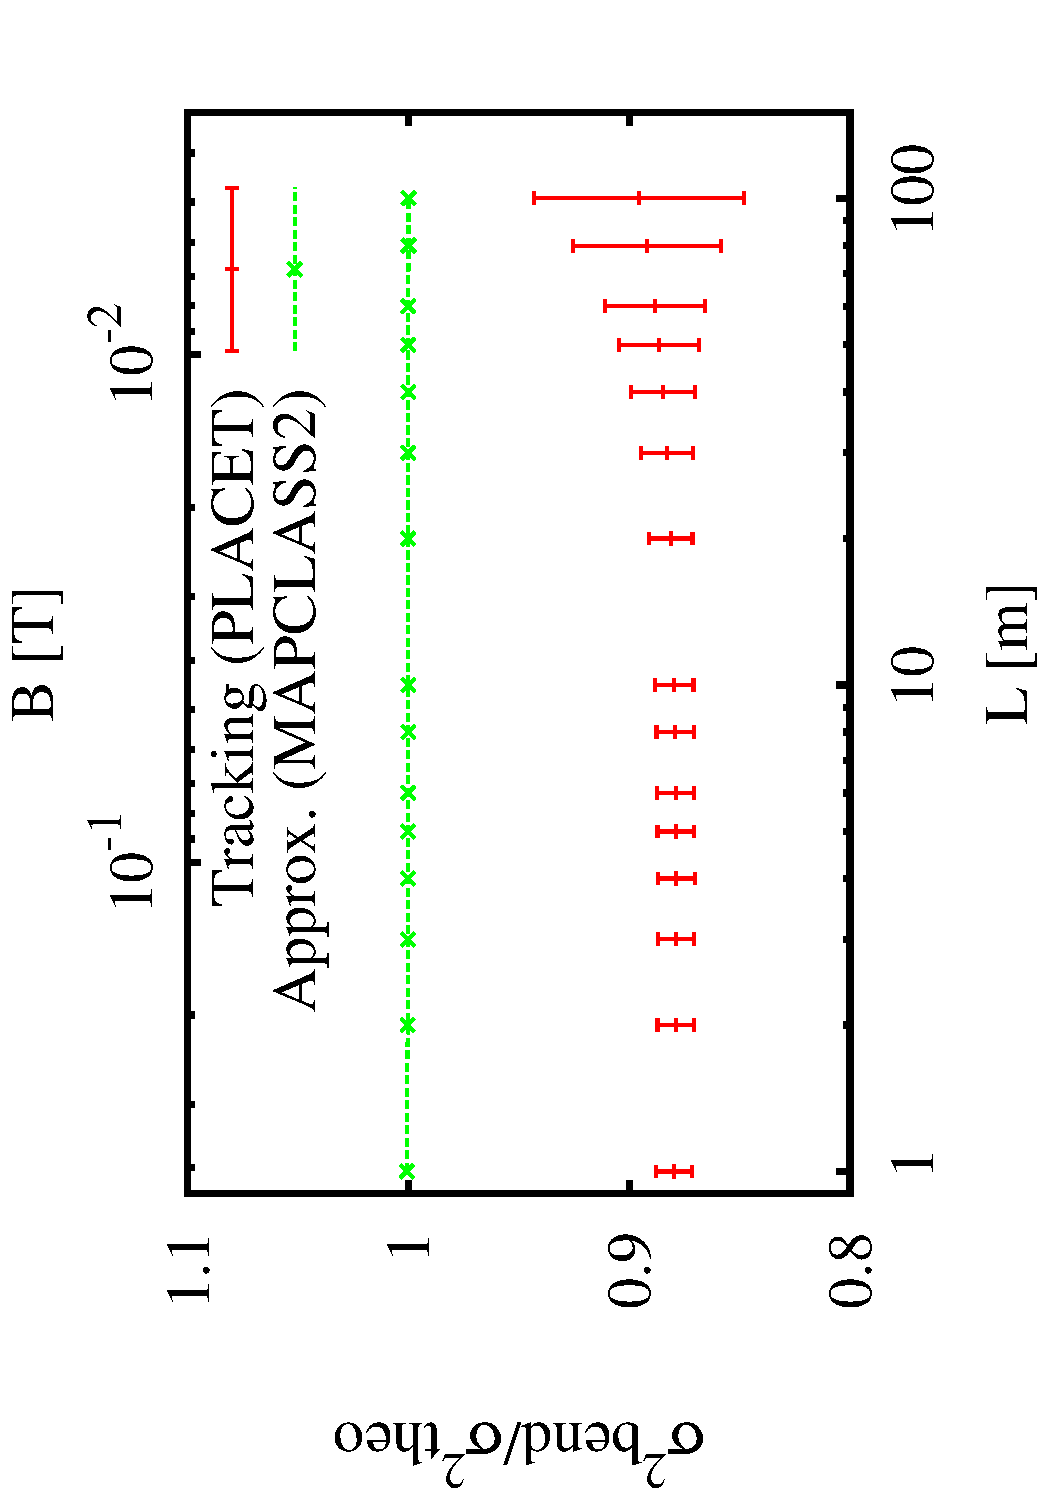
\includegraphics[scale=0.30,angle=-90]{sigma_Lbend.pdf}
  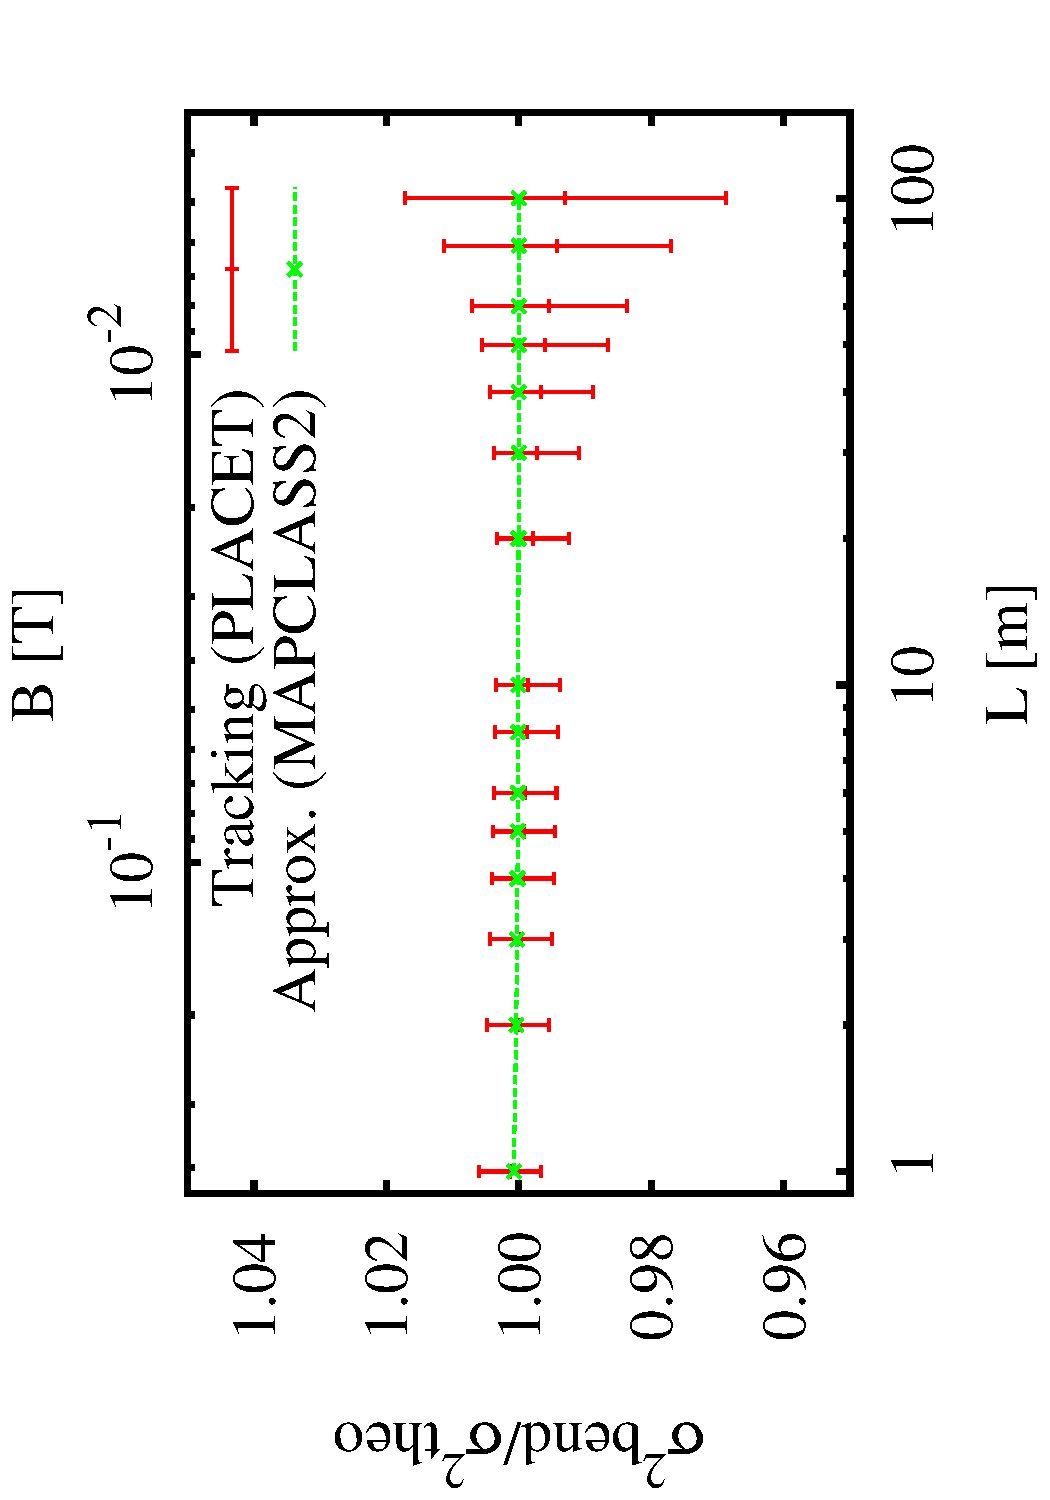
\includegraphics[scale=0.30,angle=-90]{sigma_Lbend_r6.pdf}\par
  \hspace*{1.0cm}(c)\hspace*{7.6cm}(d)\par
  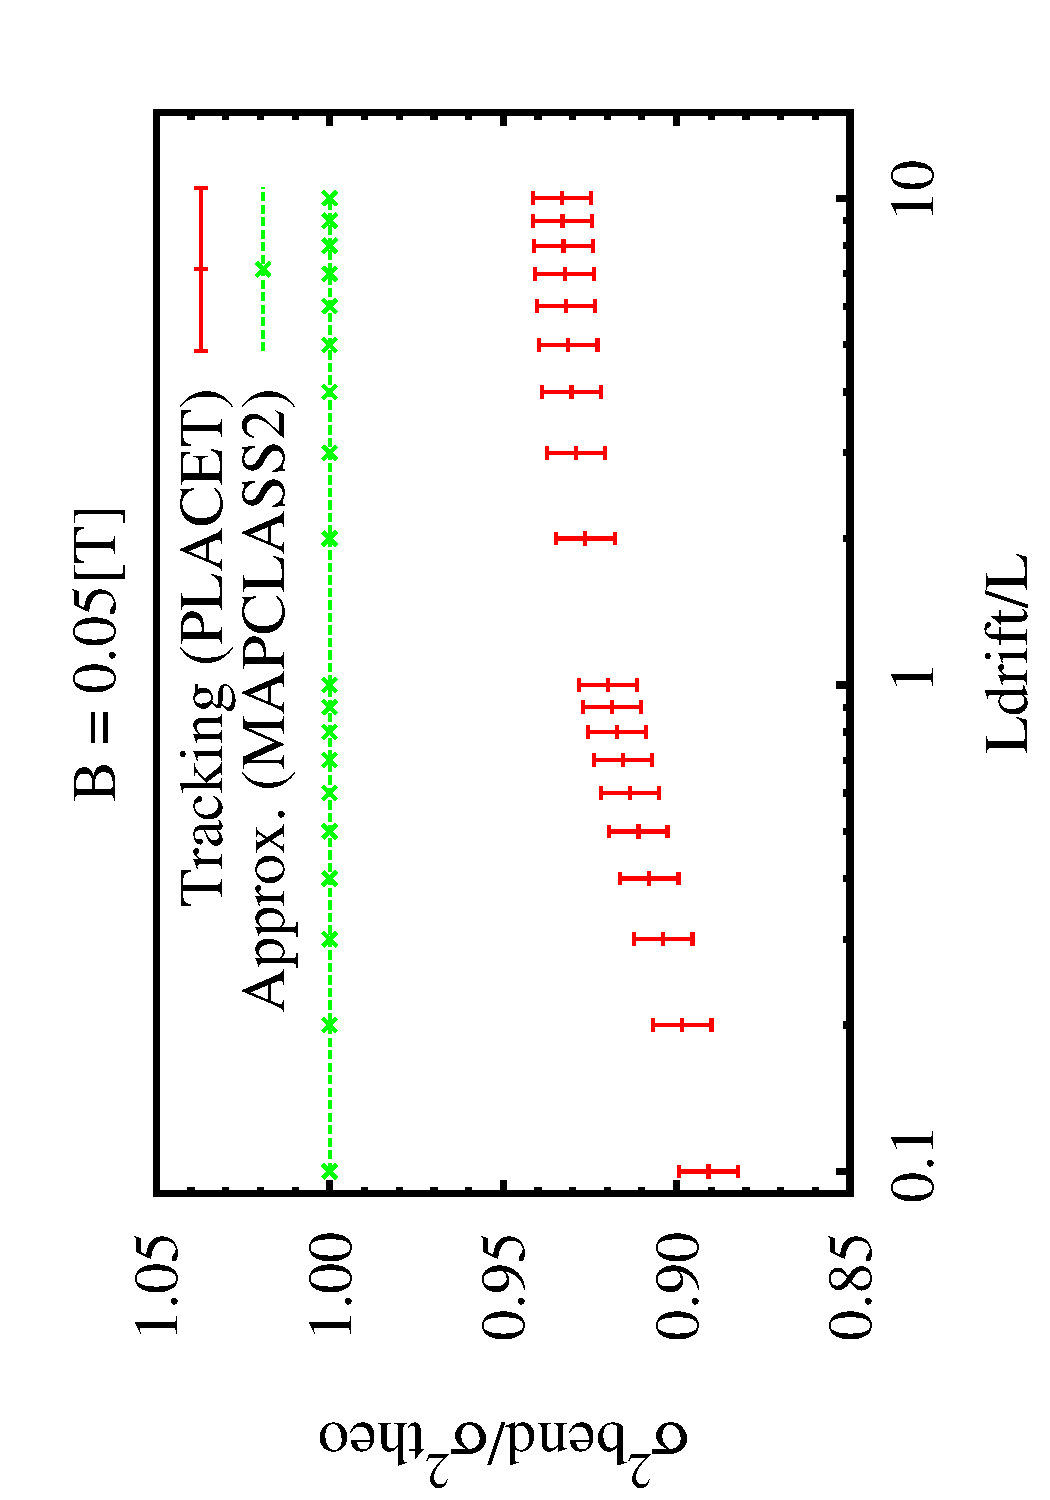
\includegraphics[scale=0.30,angle=-90]{sigma_Ldrift.pdf}
  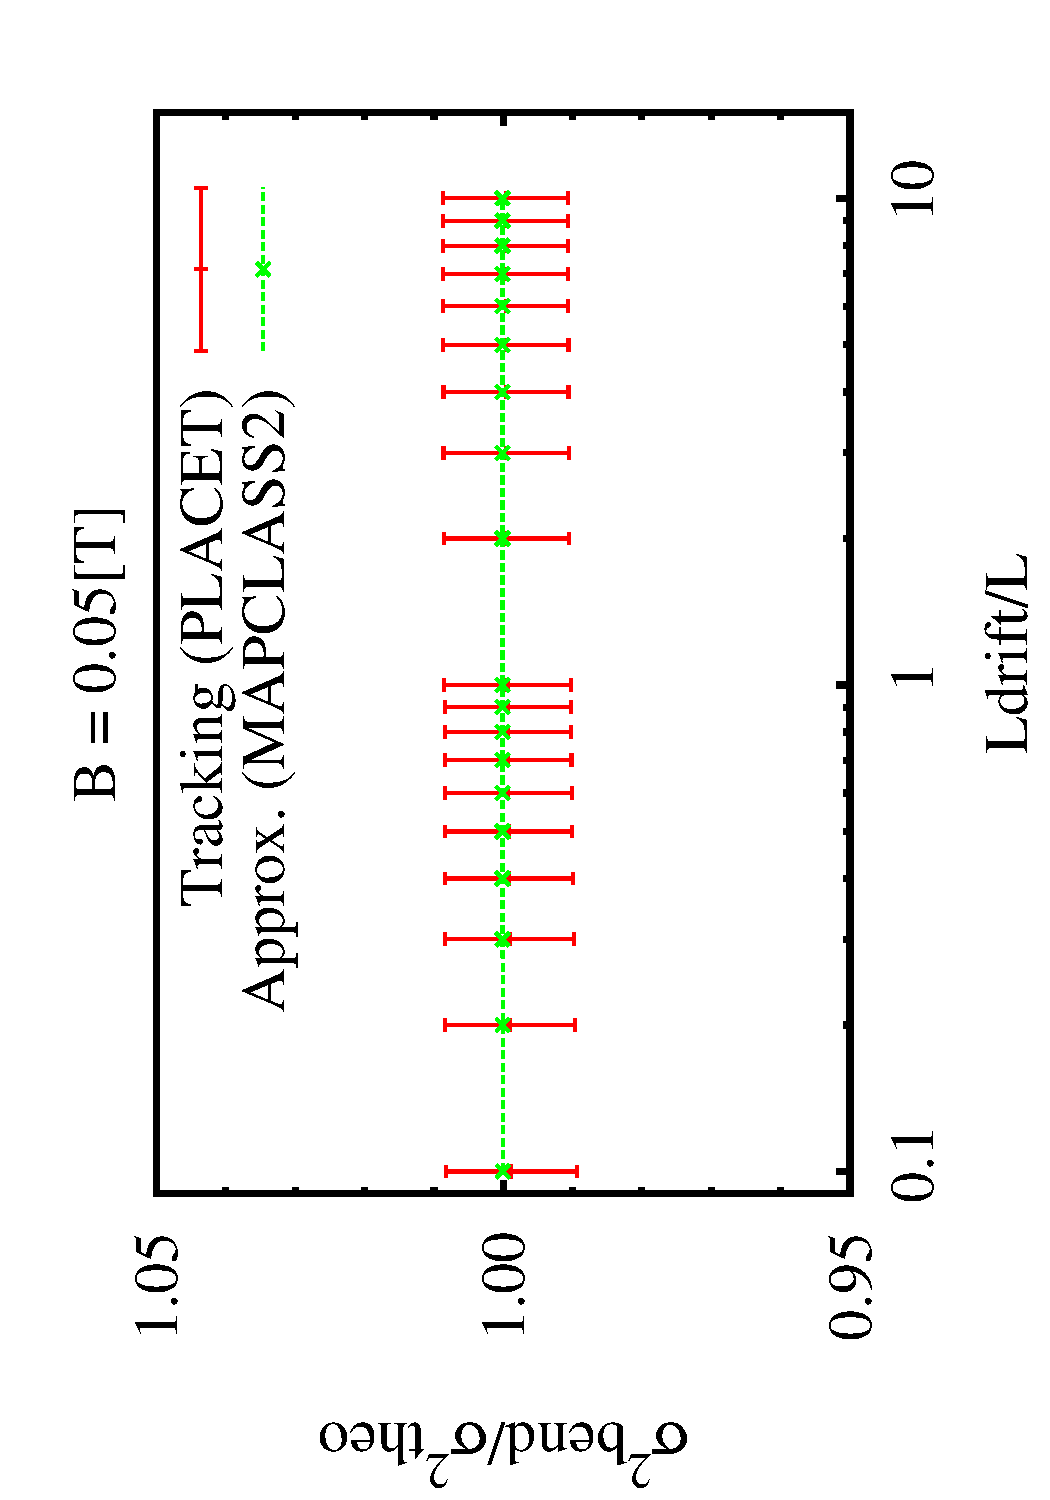
\includegraphics[scale=0.30,angle=-90]{sigma_Ldrift_r6.pdf}
  \hspace*{1.0cm}(e)\hspace*{7.6cm}(f)\par
\caption{Beam size increase due to radiation normalized to closed expression assuming negligible energy loss. (Left) `Default' radiation option, (Right) `Six\_dim' option in PLACET 0.99.01. Plots (a) and (b) correspond to $L=10$ m for a dipole only. Plots (c) and (d) correspond to $\theta=10^{-4}$ rad for a dipole only. Plots (e) and (f) correspond to $L=10$ m and $\theta=10^{-4}$ rad while varying the drift length. Beam energy is 1500 GeV in all cases.}\label{figSR}
\end{figure}
\clearpage
\section{Model limitations}\label{s:modellim}
The radiation model is valid when the average number of photons radiated per particle $\langle N\rangle$ is enough to characterize the overall effect in position by its second moment, where $\langle N\rangle  = C_1E\theta$ with $C_1=20.61\text{ GeV}^{-1}$.\par
Although, Sect. \ref{s:comparison} explores the variation of $\theta$, this also implies a change in the magnetic field strength $B$. In this Section the magnetic field is fixed $5 \times 10^{-3}$ T and the magnet length $L$ is systematically shortened to reduce the average number of photons emitted by each particle, changing $\theta$ because $B\rho$ is fixed for $E=1500$ GeV.\par
Fig. (\ref{figPhotons}) shows how the average number of photons emitted decreases with the dipole length $L$. It is visible also that the region where the average is below one photon is also the starting point when tracking and theory start to differ, reaching $\pm10\%$ max.\par
This result is equivalent to the thin dipole approximation mentioned in Sect. \ref{s:comparison}, where the dipole sectioning makes of each slice a binomial trial of photon emission, approaching the Poisson theoretical distribution for large number of slices.\par
\begin{figure}[htb]
\centering
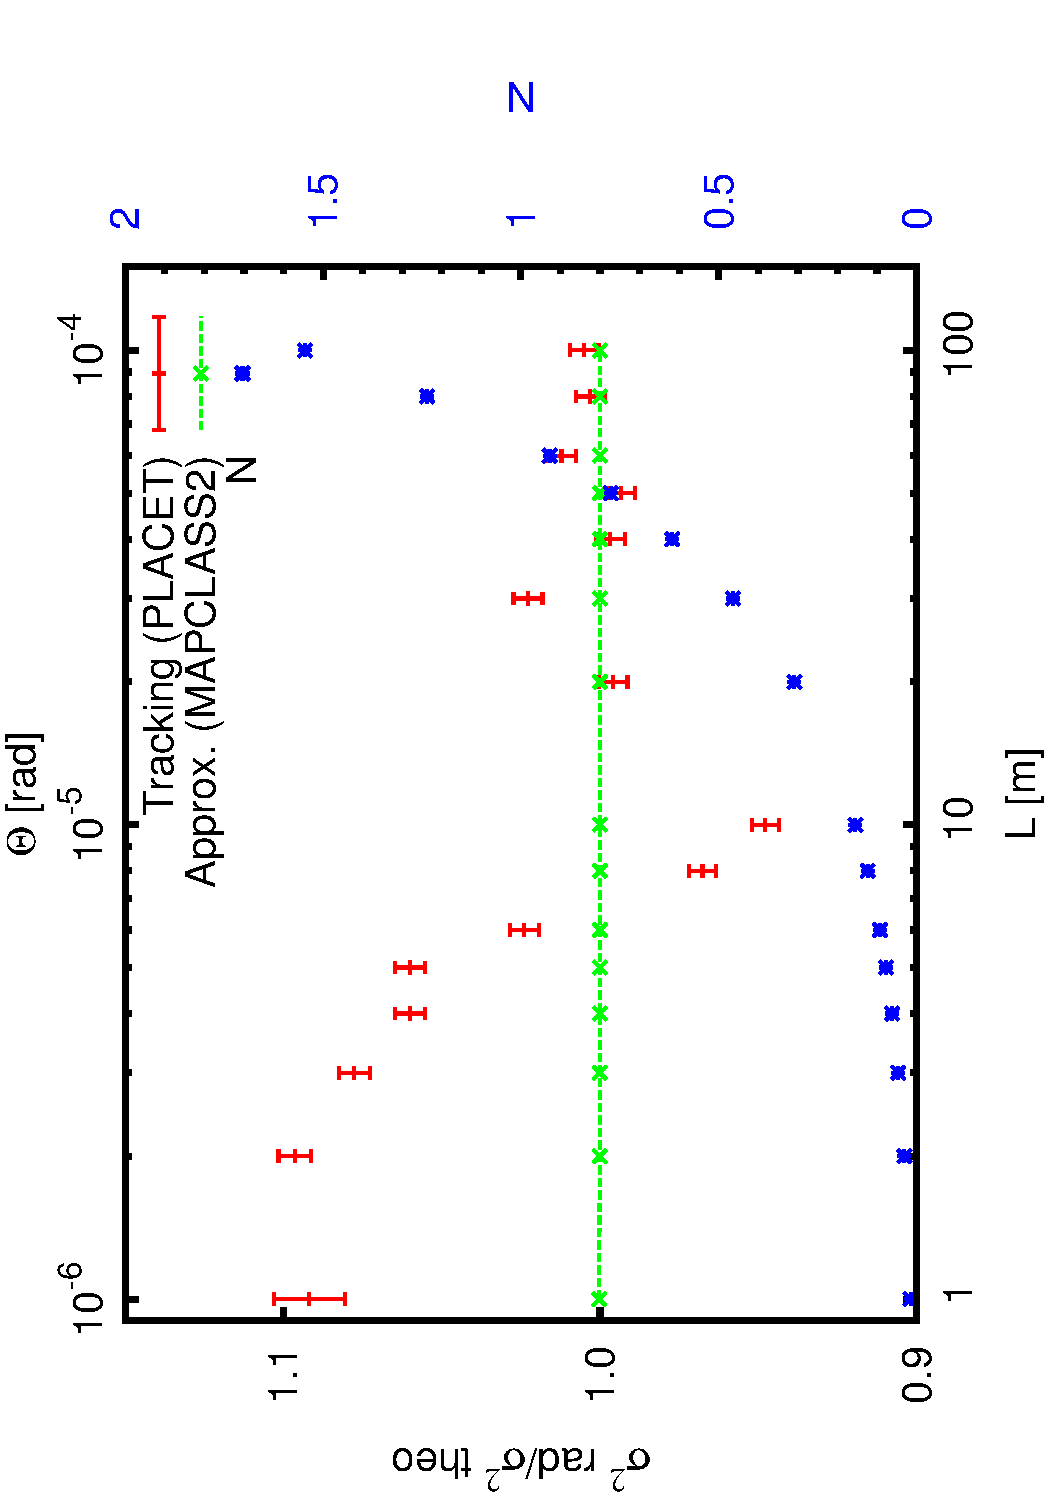
\includegraphics[scale=0.6,angle=-90]{./sigma_Bfix5e-3T.pdf} \caption{Result from tracking, closed expression with the mean number of photons emitted by particle superimposed. Magnetic field is fixed at $5\times 10^{-3}$ T and $E=1500$  GeV.}\label{figPhotons}
\end{figure}

\section{Validity for the FFS}
The CLIC FFS design is composed by magnets with bending angles shown in Table \ref{T-nphotons_3TeV} for 3 TeV and Table \ref{T-nphotons_500GeV} for 500 GeV.  The third column indicates the number of magnets used in each of those sections.\par 
Although the average value of photons emitted per magnet is low, these are grouped in long sections with common bending angle. \begin{table}[ht]
\begin{minipage}[b]{0.45\linewidth}\centering
\begin{tabular}{c|c|c}\hline\hline
 $|\theta|$ & $\langle N \rangle$&Qty.\\
 ($\mu$rad)&&\\\hline
 $\;\;$1.1& 0.07 &70 \\
 $\;\;$3.9& 0.24 &20 \\
 17.2& 1.06 &10\\\hline
\end{tabular}\caption{Bending angles in CLIC 3 TeV.}\label{T-nphotons_3TeV}
\end{minipage}
\hspace{0.5cm}
\begin{minipage}[b]{0.45\linewidth}
\centering
\begin{tabular}{c|c|c}\hline\hline
 $|\theta|$& $\langle N \rangle$&Qty.\\
 ($\mu$rad)&&\\\hline
 $\;\;\;\;$8.3& 0.08&70\\
 $\;\;$27.5& 0.28 &20\\
 135.0& 1.39 &10\\\hline
\end{tabular}\caption{Bending angles in CLIC 500 GeV.}\label{T-nphotons_500GeV}
\end{minipage}
\end{table}
Using the conclusions from Sect. \ref{s:modellim} it will be similar to the thin dipole approximation and the tracking coded should be within $\pm10\%$ agreement with the theoretical contribution from radiation in bending magnets.\par
